\section{The RADIUS System Design}\label{sec:system}
In this section, we give an overview of the system design and the architecture of RADIUS, followed by the introduction of its major functional modules. In addition, we motivate the use of Bayesian thresholding in RADIUS to achieve minimal error rate and high robustness in detecting link quality anomalies, based on a comparison with the CDF thresholding and the Chebyshev thresholding techniques.  
%In this section, we give an overview of the system design and the architecture of RADIUS, followed by the introduction of its major functional modules. In particular, we motivate the use of Bayesian thresholding in our anomaly detection system to achieve minimal detection error rate and high robustness in detecting link quality anomalies. We also compare the detection performance of Bayesian thresholding against two other detection techniques.  


%\textit{RADIUS} is featured by its low-overhead, accurate and robust anomaly detection. This is achieved by a hybrid approach that is composed of a set of distributed \textit{Detection Agents} (DA), each of which is a software module instrumented in sensor nodes to locally perform anomaly detection while being adaptive to dynamic changes and a centralized software \textit{Visualizer and Control Center} (VCC) that updates the parameter required for threshold computation in case of high detection error rate. Figure~\ref{fig:architecture} presents the architecture of the \textit{RADIUS} system. 

\subsection{RADIUS System Overview}
%To carry out the concept of RADIUS approach 
To achieve its goal, RADIUS adopts a hybrid approach. It comprises a set of distributed software modules located at the sensor nodes, which are called \textit{Detection Agents} (DAs), to detect anomalous link quality degradation along routing paths. In addition, a central server, called \textit{Visualizer and Control Center} (VCC), is used to monitor the performance of both the network and the RADIUS system. The overall system architecture of RADIUS is shown in Figure~\ref{fig:architecture}.
%To efficiently achieve accurate and robust anomaly detection in low-powered WSNs, we adopt a hybrid approach that comprises a set of distributed software modules (Detection Agents, DAs) detecting on the sensor nodes anomalous link quality changes along routing paths. In addition, a central server, called \textit{Visualizer and Control Center} (VCC), monitors the performance of both the network and the RADIUS system.  The overall system architecture is shown in Figure~\ref{fig:architecture}.



\paragraph{Two phases.} Similar to other anomaly detection systems, RADIUS runs in two phases: a training phase and an anomaly detection phase. During the \emph{training phase}, the user first observes if the performance of the network, e.g., packet delivery rate, is above the user requirement. In this case, each DA measures and collects the RSSI readings of the received packets to construct a ``normal profile'' for each monitored link, based on which a set of thresholds are generated. In the following \emph{anomaly detection phase}, each DA compares the runtime RSSI readings with the generated thresholds to detect if there is an anomalous link quality degradation. 


%\textbf{Two phases.} Similar to other anomaly detection systems, RADIUS runs in two phases: a training phase and an anomaly detection phase. During the \emph{training phase}, the user first observes if the performance of the network, e.g., packet delivery rate, is above the user requirement. In this case, each DA measures and collects the RSSI readings of the received packets to construct a ``normal profile'' for each monitored link. In the following \emph{anomaly detection phase}, each DA compares the runtime RSSI readings with the normal profile to detect if there is anomalous link quality degradation. 


\paragraph{System modules.} Choosing an appropriate anomaly detection technique is the key to achieve high detection performance, especially when using the highly varying RSSI values to distinguish the good links (with low packet losses) from weak links (with high packet losses) as accurately as possible. To tackle this problem,  RADIUS employs a thresholding technique based on the Bayes decision theory. 
%the Bayesian thresholding technique.
% to find the so-called Bayes threshold. 
Through the process of deciding a Bayes threshold, the detection error rate
% (including FPR and FNR) is mathematically guaranteed 
can be minimized, as to be discussed in Section \ref{sec:thdComputation}. In a (close to) Gaussian channel, the computation of the Bayes threshold for a desired error only relies on a user-defined parameter (i.e. the \textit{a priori} probability in the Bayes formula) and two statistical measures (i.e. the {\em mean} and the {\em standard deviation}) of the measured RSSI values. 

\begin{figure}[t]
	\centering
	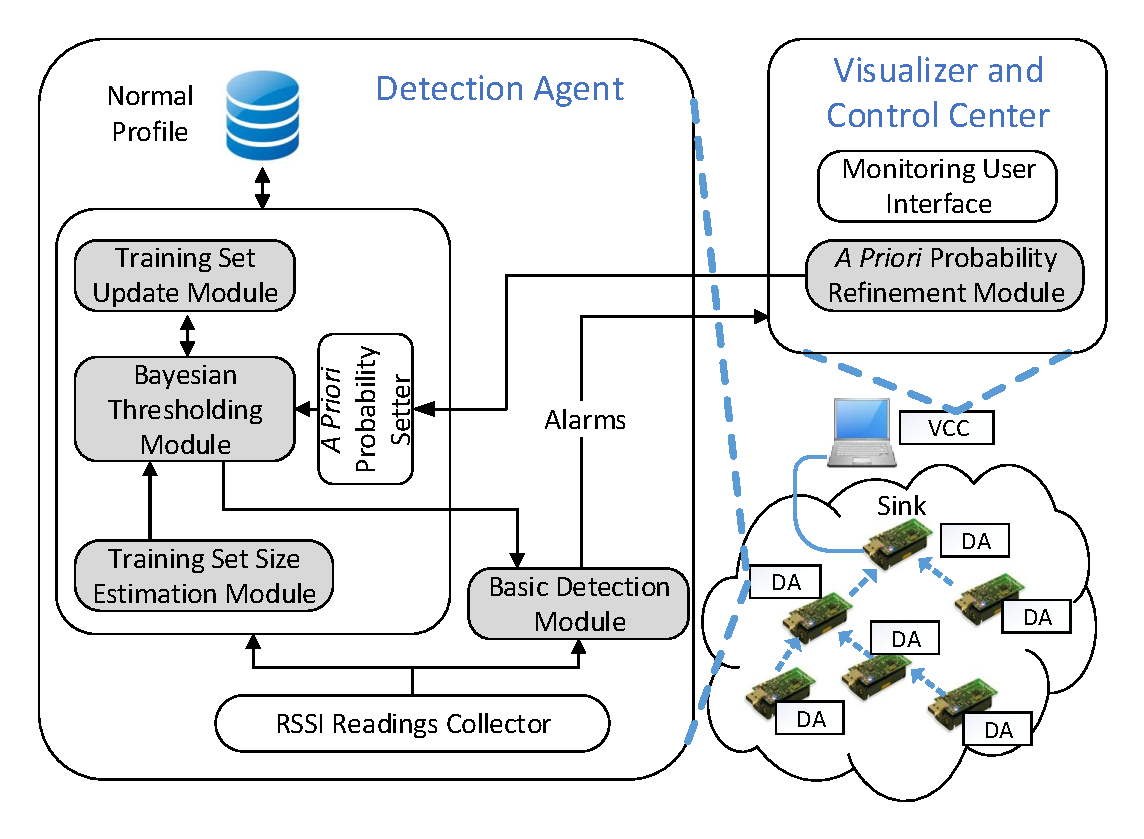
\includegraphics[width=1\linewidth]{system-architecture-new3}
	\vspace{-0.9cm}
	\caption{\textbf{The RADIUS system design and its functional modules.}}
	\label{fig:architecture}
	\vspace{-0.8cm}
\end{figure}

During the training phase, the \texttt{Bayesian Thresholding Module} in each DA constructs the RSSI profiles (mean and standard deviation) of good links, and at the end of this phase,  the module derives a Bayes threshold for each monitored link. Note that, although the detection error is minimized by employing the Bayesian thresholding technique, the detection error rate may still be high when the mean and standard deviation estimates are not accurate due to insufficient RSSI training samples. To alleviate this problem, RADIUS employs a \texttt{Training Set Size Estimation Module} before the threshold computation. In this module, we use a confidence interval to estimate for each link the number of minimal RSSI samples required to produce a good approximation of the true underlying distribution of the RSSI values and hence the mean and standard deviation. This module ensures a ``good enough'' quality of the first Bayes threshold while keeping an acceptable training set size to avoid an overly long training time. 


After the above operations, the anomaly detection phase starts. Recall that RADIUS is aimed to achieve high detection accuracy for links under diverse link conditions and be robust to environment changes. This is realized mainly by the \texttt{Basic Detection Module} and the \texttt{Training Set Update Module}. For the former, i.e. to achieve consistent high detection accuracy for different links, the system should avoid fine-tuning of the parameters involved in the thresholding, which specifically means no tuning of the \textit{a priori} probability for each individual link. For this purpose, the \texttt{Basic Detection Module} compares the runtime RSSI measurements after smoothing with the Bayes threshold to decide about whether there is an anomalous link quality degradation or not. Later in Section~\ref{sec:ThresholdChoice}, we show that a near-optimal detection accuracy is possible for all links across the network by even a coarse choice of the \textit{a priori} probability setting. In addition, to cope with dynamic environment changes, the \texttt{Training Set Update Module} is introduced, which updates the RSSI training set continuously during the detection phase in a memory-efficient way.


%After the above operations, the anomaly detection phase starts. Recall that RADIUS is aimed to achieve high detection accuracy for links under diverse link conditions and be robust to environment changes. This is realized mainly by the \texttt{Basic Detection Module} and the \texttt{Training Set Update Module}. For the former, i.e. to achieve consistent high detection accuracy for different links, the system should avoid fine-tuning of the parameters involved in the thresholding, which specifically means no tuning of the \textit{a priori} probability for each individual link. In RADIUS, the \texttt{Basic Detection Module}, together with the \texttt{Bayesian Thresholding Module}, is for this purpose, where Baysian thresholding is implemented which compares the Bayes threshold with runtime RSSI measurements after smoothing to detect link quality anomalies. Later in Section~\ref{sec:ThresholdChoice}, we show that a near-optimal detection accuracy is possible for all links across the network by even a coarse choice of the \textit{a priori} probability setting. In addition, to cope with dynamic environment changes, the \texttt{Training Set Update Module} is introduced, which updates the RSSI training set continuously during the detection phase in a memory-efficient way.

To further explore the potential of the \textit{a priori} probability parameter in achieving or maintaining the high detection accuracy, a feedback-based \textit{a priori} probability adaptation technique is introduced in RADIUS during the anomaly detection phase through the \texttt{A Priori Probability Refinement Module}. If the module in the VCC observes that the error rate of RADIUS for a link increases above a certain threshold, it then informs the \textit{Setter} at the DA to tune the setting of the \textit{a priori} probability.



%To further explore the potential of the \textit{a priori} probability parameter in achieving or maintaining the high detection accuracy, a feedback-based \textit{a priori} probability adaptation technique is introduced in RADIUS during the anomaly detection phase, through two more RADIUS modules: the \texttt{A Priori Probability Setter} module and the \texttt{A Priori Probability Refinement Module}.  The former at each DA tunes the setting of the \textit{a priori} probability if the latter in the VCC observes that the detection error for a link increases above a certain threshold. 
 
%Another important feature of RADIUS is the high detection accuracy can be achieved under diverse link conditions while being robust to environment changes. In order to adapt to environment changes, the \texttt{Training Set Update Module} updates the RSSI training set continuously during the detection phase in a memory-efficient way without incurring high memory overhead. To achieve high accuracy under diverse link conditions, an anomaly detection system should avoid fine-tuning of the parameters involved in the thresholding technique. In our case, this means no tuning of the \textit{a priori} probability for each individual link. In Section~\ref{sec:ThresholdChoice}, we show that a near-optimal detection accuracy is possible for all used links with a coarse choice of the \textit{a priori} probability setting. In addition, a feedback-based \textit{a priori} probability adaptation technique is introduced in RADIUS to maintain the high detection accuracy over time. The \texttt{Setter} at each DA tunes the setting of the \textit{a priori} probability if the \texttt{A Priori Probability Refinement Module} in the VCC observes that the detection error for a link increases above a certain threshold. 

%Note that although VCC is a centralized unit to control the execution of the system, the detection of link quality degradation alone does not rely on VCC and is fully distributed.

In summary, the DA on each sensor node monitors the link quality of the links used by the higher-layer network protocols and fire alarms to inform the VCC and the network administrator about detected anomalous link quality degradations. In the training phase, when the network performance satisfies the user requirements, each DA generates locally the best RSSI threshold using Bayesian thresholding (Section~\ref{sec:thdComputation}) for each monitored link after collecting enough samples as determined by the minimal training set size estimation (Section~\ref{sec:minTrainingSet}). In the detection phase, using the generated thresholds, each DA performs local detection including data smoothing (Section~\ref{sec:dataSmoothing}) and adaptively adjusts the threshold either with local information updating the training set (Section~\ref{sec:trainingSetUpdate}) or with the refinement of the \textit{a priori} probability by the feedback from the VCC (Section~\ref{sec:prioriRefinement}) to achieve high accuracy and robustness.
% at the same time.
%Details of each employed technique in RADIUS are presented in Sec. \ref{sec:approach}.

\paragraph{Remarks.} In RADIUS, we have focused on using the RSSI link attribute to detect anomalous link quality degradation. However, its approach is not strictly limited to using RSSI, which may be extended to use other communication attributes as potential indicators of (possibly other types of) network performance anomalies. For instance, \textit{packet CRC error rate} could be observed for identifying packet collisions, \textit{packet overflow rate} for indicating queuing losses, and \textit{packet inter-arrival time} for determining node crashes. %Applicability
%\textbf{Remarks:} In this work, we apply the RADIUS approach to the RSSI link attribute for detecting anomalous link quality degradation. However, the approach is not strictly limited to the analysis of RSSI and it can also be applied to alternative communication attributes as potential indicators of other types of network performance anomalies. E.g., \textit{packet CRC error rate} could be observed for identifying packet collisions, \textit{packet overflow rate} for queuing losses and \textit{packet inter-arrival time} for determining node crashes. %Applicability

\subsection{Motivation of Bayesian Thresholding} \label{sec:motivationBayes}

Before describing the details of the Bayesian thresholding technique, we first motivate and illustrate its need. Its ability to deal with the challenge of achieving minimized detection error in a noisy channel is then evaluated in comparison with the CDF-based (or Percentile-based) and Chebyshev inequality-based thresholding techniques.

\subsubsection{Achieving Minimal Detection Error} \label{sec:problem}
	
Due to its stochastic nature, the quality of a WSN link can vary randomly. To illustrate this, Figure \ref{fig:PIMRC-RSSI} presents two RSSI traces collected from a real WSN link. The upper one is when the link operated in a normal state with a packet delivery ratio (PDR) higher than 99\% (i.e. good link), while the lower one is when the link operated in an abnormal state with PDR below 52\% (i.e. weak link). The figure also shows that the two clusters of RSSI values, although mostly centred around their respective means, partially overlap with each other and no threshold can clearly discriminate them. This is due to the stochastic nature and the well-known temporal properties of low-power wireless links \cite{2893729}. 


An implication of Figure \ref{fig:PIMRC-RSSI} is that no single RSSI threshold can, based on an RSSI value, lead to a definite conclusion without error if the link is in the good or weak state. Our objective is to find a threshold that minimizes the misidentification error. As shown in the figure, finding such a threshold involves a tradeoff decision to balance between reducing the chance that a good link is misidentified as a weak link and reducing the chance that a weak link is falsely viewed as a good link. The former is called false positive rate (FPR) and the latter called false negative rate (FNR). 

Mathematically, such a decision problem of finding the best threshold minimizing the error rate has been comprehensively studied under the Bayesian decision theory. In addition, if the monitored attribute is a Gaussian random variable (e.g., RSSI in a Gaussian channel), the complexity of Bayesian thresholding decreases significantly, falling within the limited capability of sensor nodes. This motivates our adoption of Bayesian thresholding in RADIUS. 
%Details of applying Bayesian thresholding to our problem are presented later in Sec. \ref{sec:thdComputation}. 

\begin{figure}[t]
	%\vspace{-0.2cm}
	\centering
	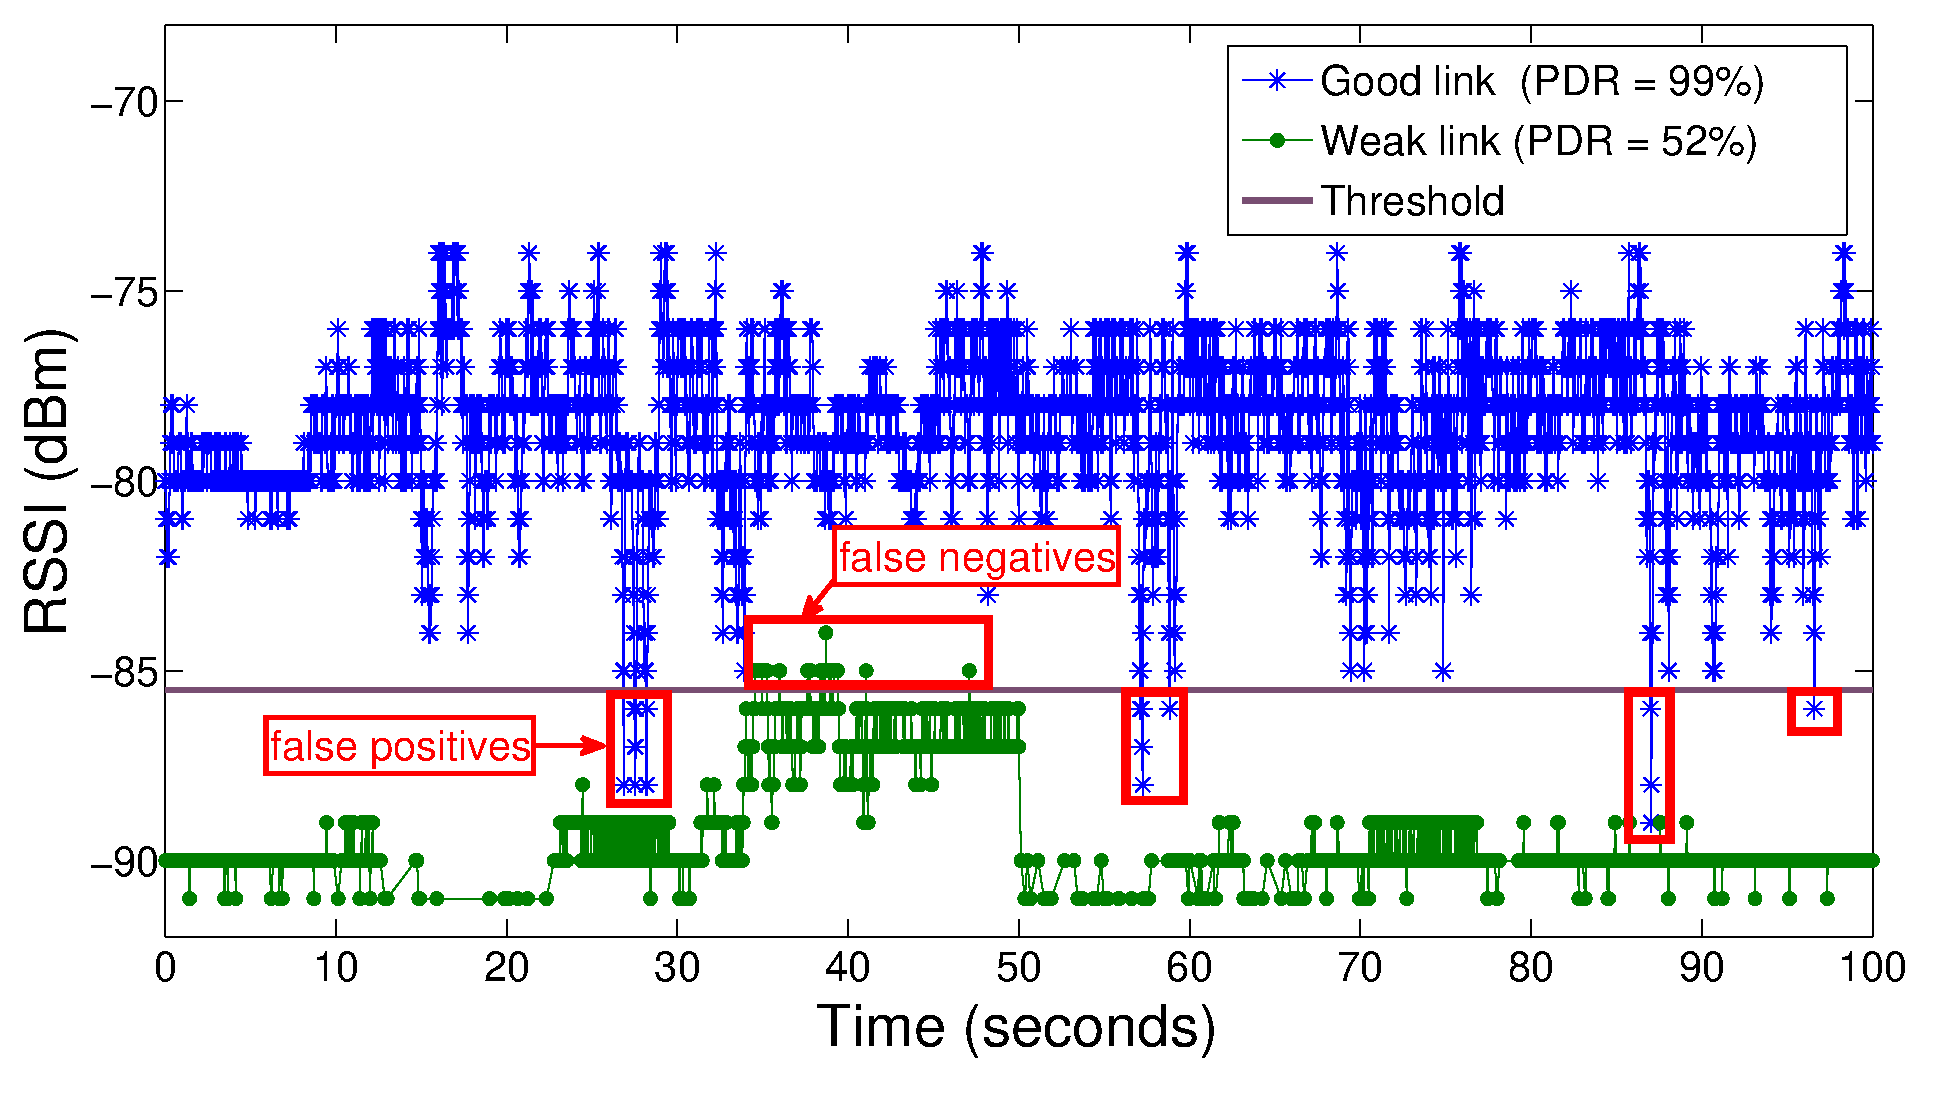
\includegraphics[width=1\linewidth]{PIMRC-RSSI}
	\vspace{-0.9cm}
	\caption{\textbf{The overlapping RSSI traces of a good link and a weak link implies that achieving high detection accuracy requires to minimize both the false positive and false negative rate.}}	
	\label{fig:PIMRC-RSSI}
	\vspace{-0.7cm}
\end{figure}

\begin{figure*}[t]
	\centering
	%\vspace{-0.5cm}
	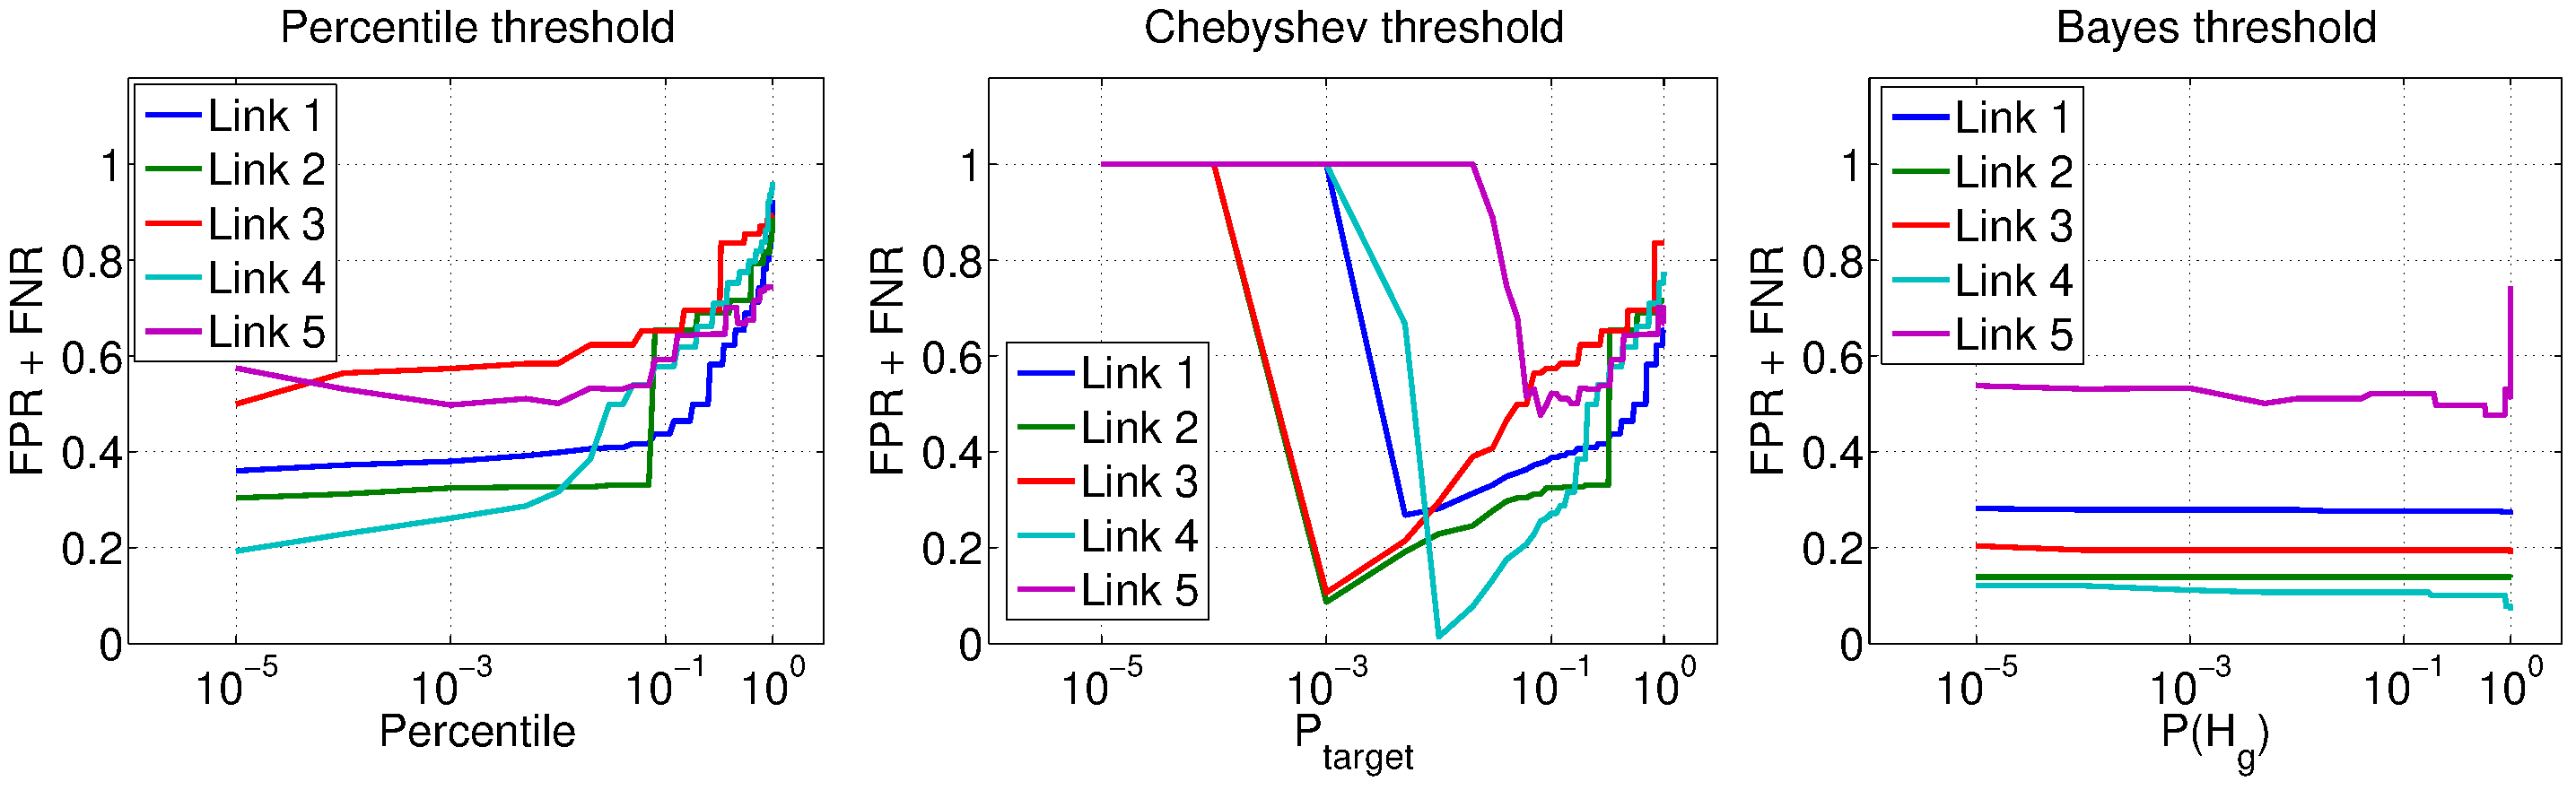
\includegraphics[width=1.0\linewidth, height = 4.5cm]{5-Compare_threshold_methods}
	\vspace{-0.7cm}
	\caption{\textbf{The performance of CDF (Percentile) and Chebyshev thresholding varies dramatically depending on the parameter setting. Instead, the performance of Bayesian thresholding is robust, providing near-optimal accuracy under different link conditions with a coarse $P(H_g)$ setting.}}
%Bayes threshold achieves higher detection accuracy than Percentile threshold while its performance is more robust than that of Chebyshev threshold.}
	\label{fig:EVA-ThdCompare}
	\vspace{-0.55cm}
\end{figure*}


\subsubsection{Comparison among Thresholding Techniques}


%Depending on the thresholding schemes, defining a threshold typically requires one or several user-defined parameters. The choice of the thresholding techniques and their parameter settings is often an important factor that determines the level of performance of the threshold-based approaches.

%To show that our Bayes thresholding is robust and less sensitive to it parameter setting, we create an example for detecting low RSSI anomaly using the Bayes thresholding and compare its detection performance  with those of two popular thresholding techniques that are often used in the literature. We particularly focus on the effect of their parameter choices on the detection performance. The comparison is based on the results of the basic thresholding without other supporting techniques for adaptation. In the following, we first introduce the related work using these two thresholding techniques and then we present the results of the comparison.

%The statistical detection scheme proposed in \cite{1515559} maintains for each sensor node the normal traffic profile on its one-hop neighbor nodes, with which anomaly can be identified. Each node maintains a received buffer to record a large set of packet inter-arrival times and an intruder buffer to record a small set of recent packet inter-arrival times. Abnormal traffic pattern is detected if satisfies
%\setlength{\belowdisplayskip}{4pt} \setlength{\belowdisplayshortskip}{4pt}
%\setlength{\abovedisplayskip}{4pt} \setlength{\abovedisplayshortskip}{4pt}
%\begin{equation*} %\label{equ:trafficAnomaly}
%|{mean(recBuff)} - {mean(intBuff)}| > {K} \cdot {std(recBuff)}
%%{N_{ts}} = {\left(\frac{z\cdot \sigma_p }{E_{\mu}}\right)}^{2}
%\end{equation*} 
%where ${K} \cdot {std(recBuff)}$ is a threshold and $K$ is a user-defined constant, the value of which impacts on the detection performance.

To illustrate the high accuracy and robustness achieved by a Bayesian thresholding based detection system,  we compare the detection performance of Bayesian thresholding with that of two aforementioned popular statistical detection techniques in WSNs: CDF-based and Chebyshev-inequality based thresholding techniques, both of which have similar complexity as the Bayesian thresholding technique.  

In a CDF-based (or Percentile-based) detection scheme, the threshold is typically defined as the \textit{x-th} percentile of the underlying data distribution of the monitored attribute. For a Gaussian channel, the resulting threshold depends on the mean and standard deviation of the collected RSSI samples as well as on a parameter setting of the \textit{percentile} defined by the user.  The other thresholding technique often used in the literature of WSNs is the Chebyshev-inequality based technique.
%, especially when the underlying probability distribution of the monitored attribute is not known as \textit{a priori}. 
In this case, the threshold is defined as follows:
\setlength{\belowdisplayskip}{3pt} \setlength{\belowdisplayshortskip}{3pt}
\setlength{\abovedisplayskip}{3pt} \setlength{\abovedisplayshortskip}{3pt}
\begin{equation}\label{equ:chebyTHD}
T_{cheby} = \overline{m} +  \sigma_m \ast \sqrt{\frac{1-P_{target}}{P_{target}}},
\end{equation}
where, in addition to the mean ($\overline{m}$) and standard deviation ($\sigma_m$) of the monitored attribute $m$, $P_{target}$ is a user-defined parameter for the desired false positive rate. Similarly, the Bayes threshold for Gaussian random RSSI depends on the same statistical measures (mean and standard deviation) as the CDF and Chebyshev methods and hence incurs a similarly low computation and memory overhead. The main difference is the parameter involved in the computation of the Bayes threshold: the \textit{a priori} probability of a link being in a good state ($P(H_g)$, as to be discussed in Section \ref{sec:thdComputation}).

% The threshold for attribute \textit{m} by applying the Chebyshev's inequality is defined as follows. 
% \setlength{\belowdisplayskip}{3pt} \setlength{\belowdisplayshortskip}{3pt}
% \setlength{\abovedisplayskip}{3pt} \setlength{\abovedisplayshortskip}{3pt}
% \begin{equation}\label{equ:chebyTHD}
% T_{cheby} = \overline{m} +  \sigma_m \ast \sqrt{\frac{1-P_{target}}{P_{target}}}
% \end{equation}
% Where $P_{target}$ is a user-defined parameter for desired false positive rate.  


For this comparison, we evaluate the system performance in terms of accuracy and robustness, with a focus on how the performance is influenced by the user-defined parameters, namely the \textit{x-th percentile} for CDF thresholding, $P_{target}$ for Chebyshev thresholding and $P(H_g)$ for Bayesian thresholding. The preferable technique is the one whose best detection accuracy performance is least sensitive to its parameter choice. Ideally, such a technique does not require fine-tuning of its parameter to achieve consistently optimal accuracy. 

We apply these three techniques individually to the same data traces collected from 5 different links in a network. The links are selected in such a way that diverse link conditions (e.g., line-of-sight,  non-line-of-sight, no human movements or frequent movement etc.) are captured. We record the false positive rate (FPR) and false negative rate (FNR) for each technique. A detection decision is considered as false positive (false negative) when the technique declares that an RSSI anomaly is detected (not detected) while the packet delivery rate over the link is above (under) a minimum (e.g., 80\%). The values of the above parameters of each method are varied in the same wide range of [$10^{-5}$, $1-10^{-5}$]. The resultant overall detection error rate (sum of FPR and FNR) for the three methods are presented in Figure \ref{fig:EVA-ThdCompare}.
	
From Figure \ref{fig:EVA-ThdCompare}, we can clearly see that the system performance with the Bayes threshold is consistently \textit{robust} for different links and is \textit{insensitive} to the value of $P(H_g)$ unless $P(H_g)$ is approaching the extreme, i.e., 1. 
%This observation validates the analysis of the effect of $P(H_g)$ in Sec. \ref{sec:ThresholdChoice}. 
In contrast, the system performance of both Percentile-based and Chebyshev-based approaches dramatically varies with changing parameter values. Furthermore, the optimal $P_{target}$ for Chebyshev threshold with minimal detection error varies significantly from link to link. Instead, Bayesian thresholding with a global coarse setting of $P(H_g)$ (e.g., any value from 0.1 to 0.9) for the analyzed 5 links provides close to the minimal detection error achieved by the Chebyshev thresholds. Finally, the accuracy with the Percentile threshold is in general worse than that with the Bayes threshold for every link with any parameter setting. 

An implication is that while CDF thresholding tends to provide tight RSSI bounds of good links for achieving a low FNR, it can easily cause a significantly high FPR in case of high randomness and temporal variations, making the technique difficult to achieve a low error rate. In addition, while Chebyshev thresholding can reach high detection accuracy, its performance highly depends on the choice of $P_{target}$. Bayesian thresholding, on the other hand, is designed to minimize the detection error while at the same time it can use a single setting of the threshold parameter $P(H_g)$ for the entire network, thus avoiding parameter tuning for every individual link. Thanks to such features, we employ Bayesian thresholding as the core detection technique in RADIUS. Details of Bayesian thresholding and the supporting techniques needed to use it are described in the following section.


